\chapter{Linear approach}
\label{cha:LinearApproach}

The first approach taken to achieve the goal was a straightforward, linear approach, which subdivides the input into sub clusters until they match. Solely the principal axis of $C_1$ and $C_2$ are computed to roughly align the clusters the similarly. 

\section{General functionality}

The algorithm starts with two sets of point clouds $C_1$ and $C_2$ of an object $M$ in different poses (see figure \ref{fig:pc_2parts}). The two point clouds are iteratively subdivided into point clusters $\mathcal{C}_1 =  (C_{1,1},\ldots, C_{1,m})$ and $\mathcal{C}_2 =  (C_{2,1},\ldots, C_{2,m})$. In each iteration step two related sub clusters of $C_1$ and $C_2$ are verified to match by applying the ICP (iterative closest point), resulting in a matching error $e$. In case of $e < \tau$, two clusters are assumed to match. Otherwise, the algorithm is applied recursively and the sub clusters are again subdivided. The algorithm terminates if all resulting sub clusters of $C_1$ can be matched to all sub clusters of $C_2$. Subsequently, they are stored depending on their location and then checked to be merged, in case of having divided a rigid part. After that step, the resulting clusters are assigned to rigid parts $\mathcal{P} =  \{P_1,\ldots,P_n\}$.

\subsection{Detecting point clusters}

As a first step, all point clusters $\mathcal{C} = \{C_1, \ldots , C_m\}$ are detected by applying region growing on all points of $M$. A cluster $C_i$ is grown from an unclustered point $\boldsymbol{p}_i(x,y)$. Another point $\boldsymbol{p}_j(x,y)$ is added to the cluster $C_i$ if the euclidean distance between them $d(\boldsymbol{p}_i, \boldsymbol{p}_j)$ is below a predefined threshold $\tau$. This threshold is thereby depending on the resolution and density of $M$. All points of $C_i$ are then iteratively compared to the remaining unclustered points to allow the cluster to grow. Once, all points of $C_i$ have been treated, another unclustered point is used as a seed. If there are no unclustered points left, the clusters with the highest number of points $n$ are selected as input clusters $C_1$ and $C_2$ (see figure \ref{fig:pc_2parts}). As a result, the remaining clusters are classified as noise and rejected for further computations.
%%
% TODO: picture of removing outliers + change notation (C1, C2)
%%
\begin{figure}[htbp]
	\centering\small
	\begin{tabular}{cc}
		\fbox{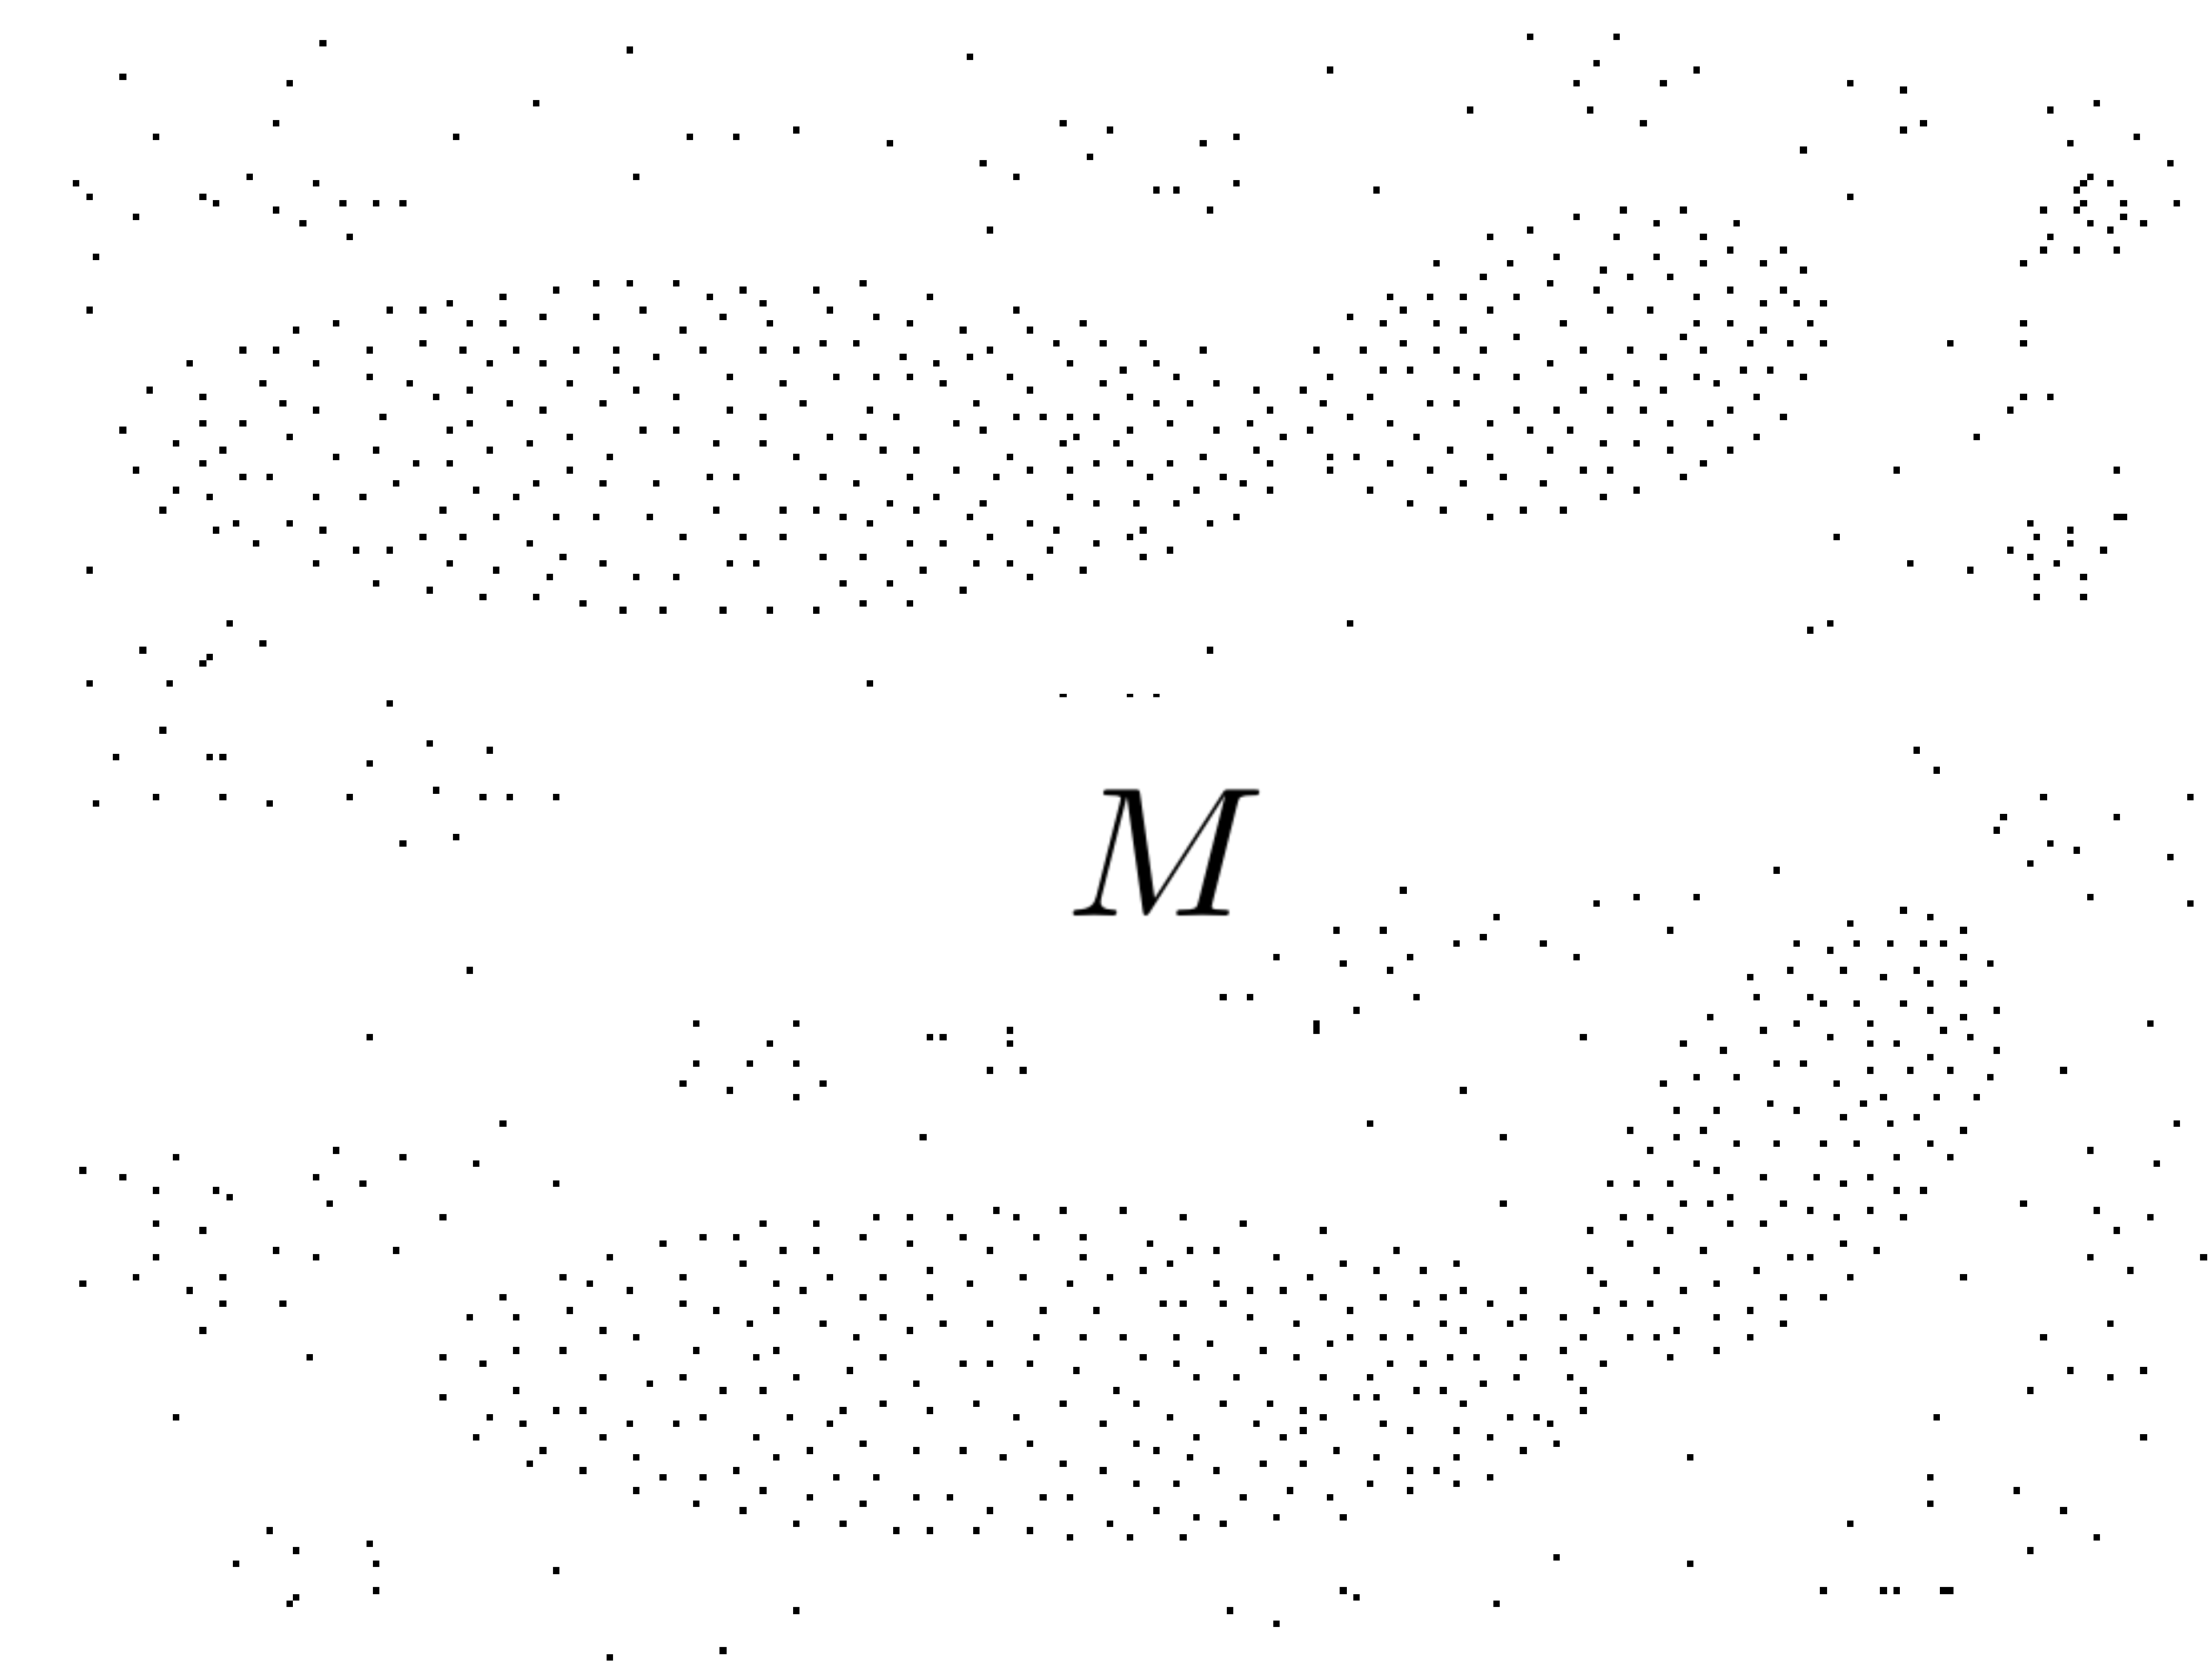
\includegraphics[width=0.45\textwidth]{pc_2parts_Noise}} &		
		\fbox{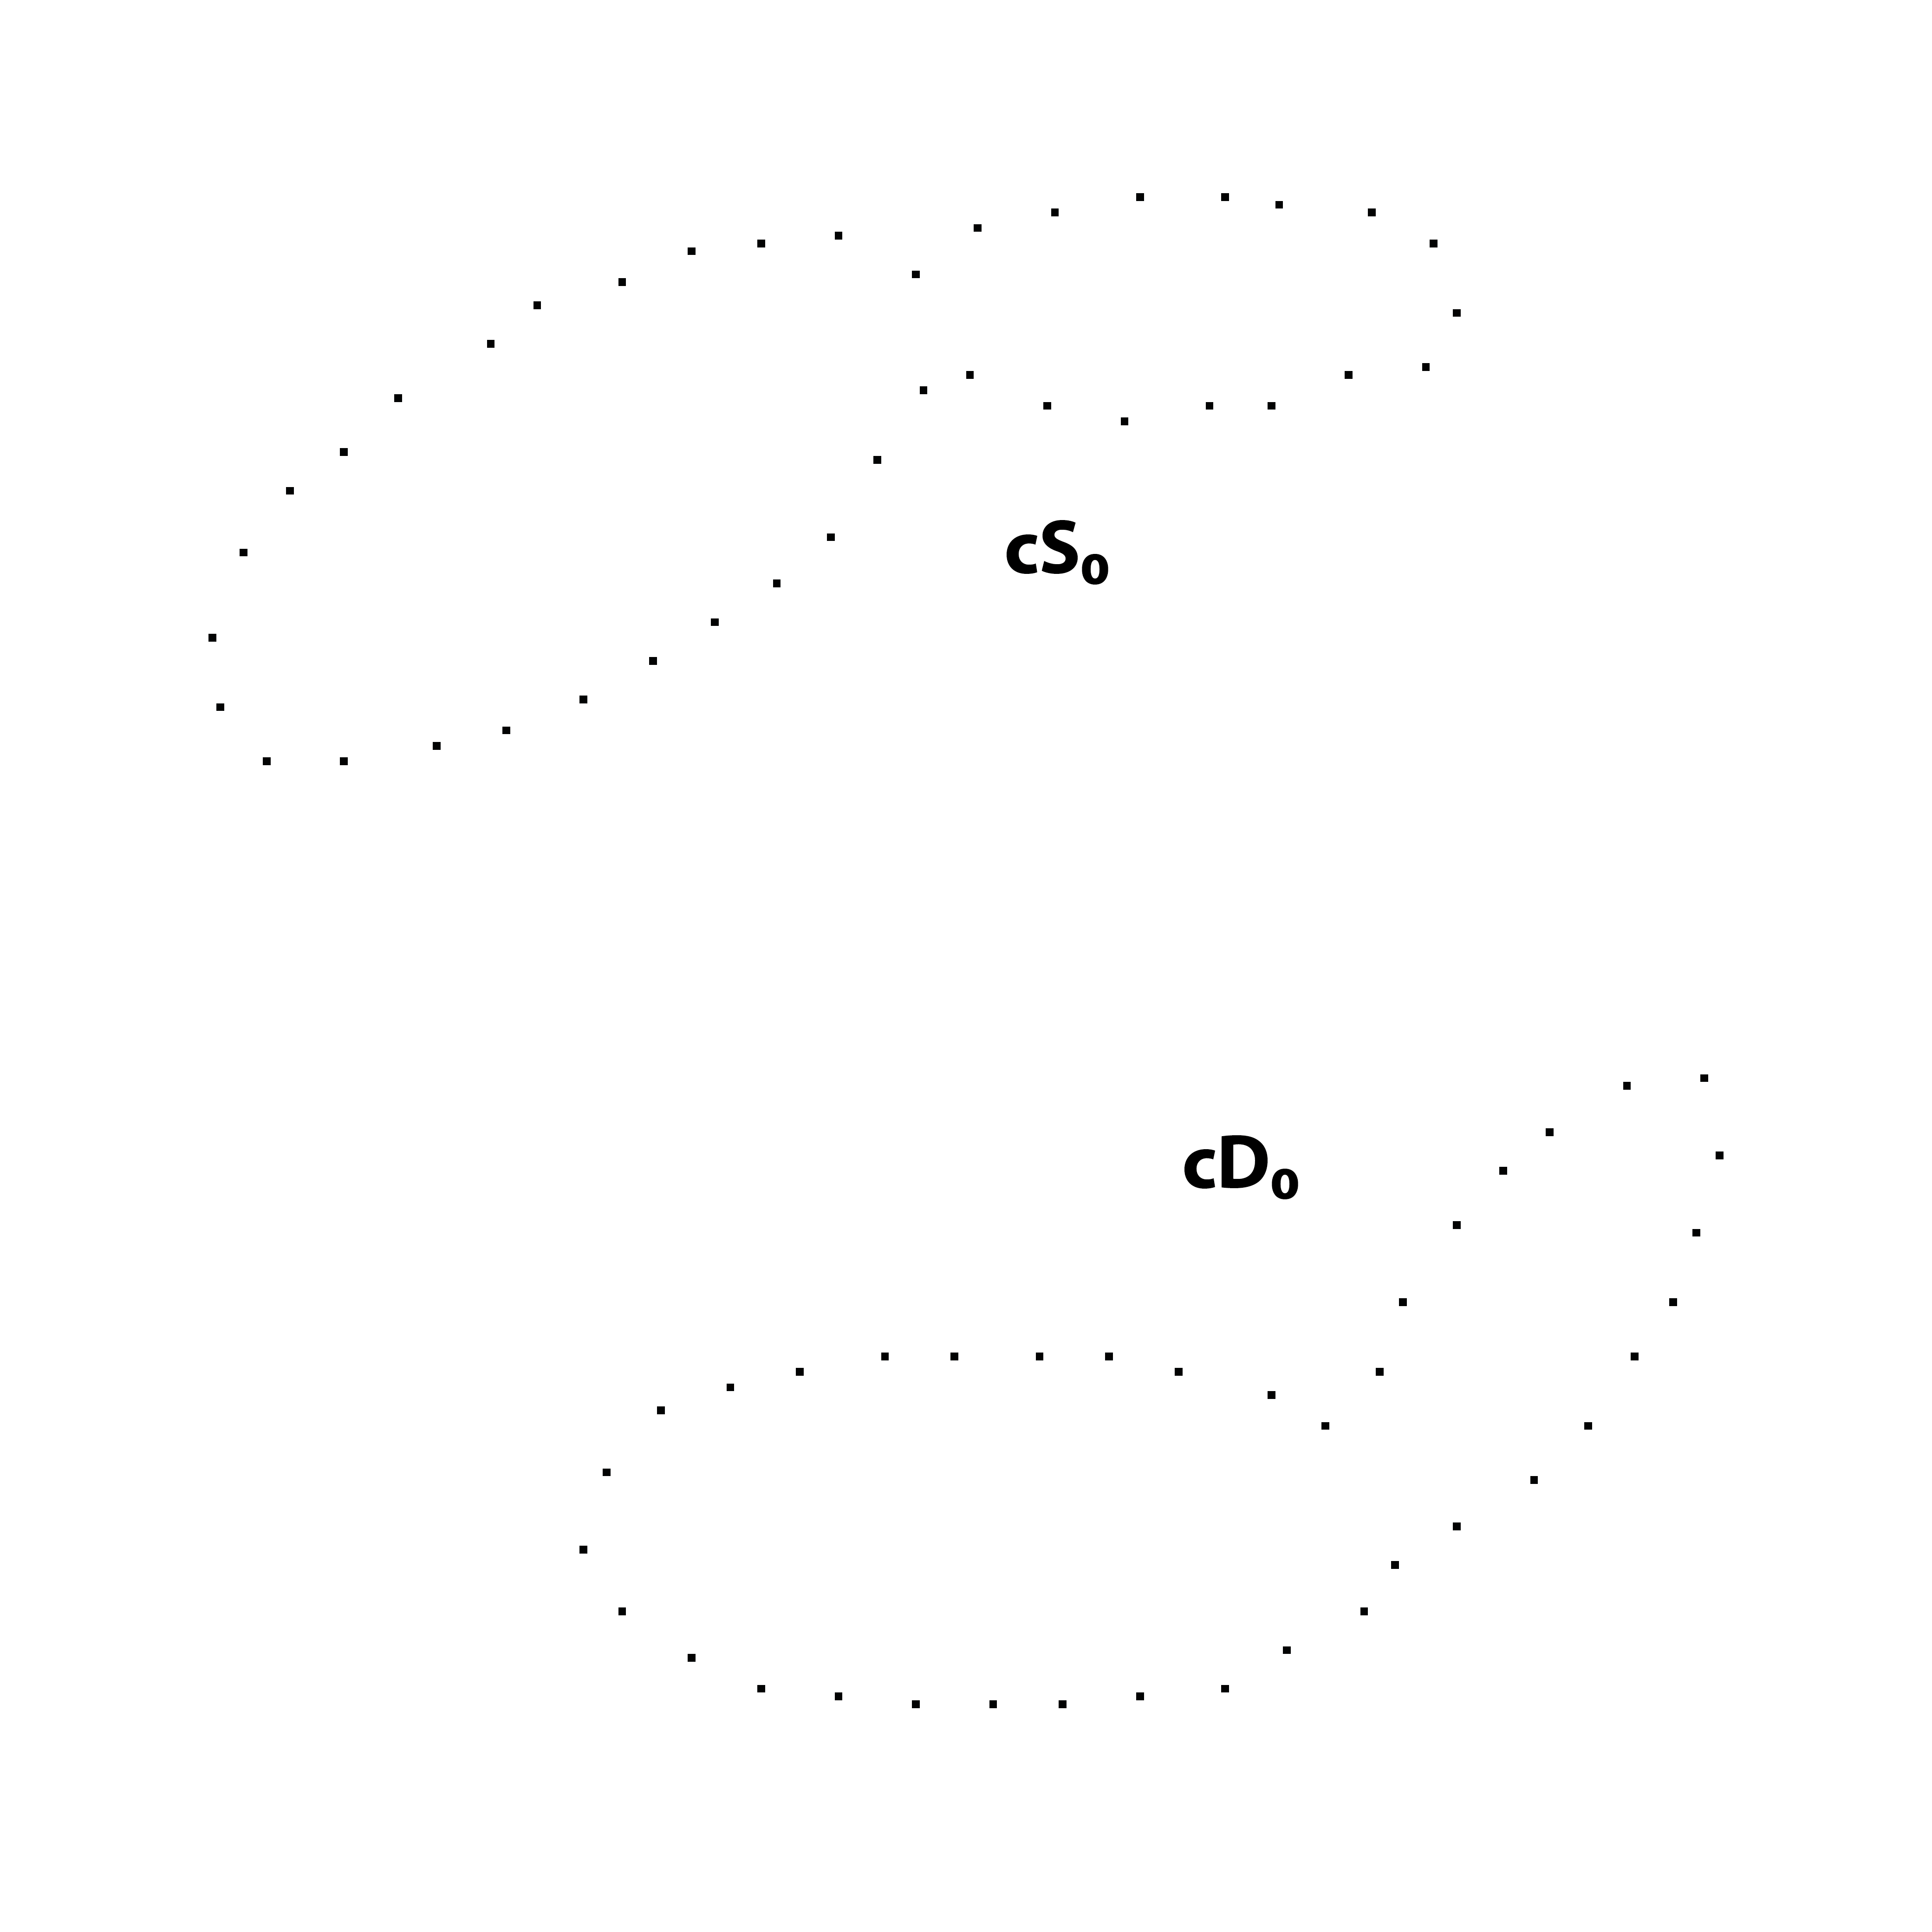
\includegraphics[width=0.45\textwidth]{pc_2parts_noNoise}} 
		\\
		(a) & (b) 
	\end{tabular}
	\caption{Taking a mesh $M$ in two different poses as input (a), removing noise of the input point clouds (b) to achieve the input clusters $C_1$ and $C_2$.} 
	\label{fig:pc_2parts}
\end{figure}

\subsection{Subdividing into clusters}
\label{Subdividing}

As a next step, the two main clusters $C_1$ and $C_2$ are taken as input for further computation steps. If the matching between two clusters does not succeed, they are both subdivided into two sub clusters. Otherwise, no subdividing is done. The whole procedure is repeated recursively for all clusters $\mathcal{C} = (C_{i,1}, \ldots, C_{i,m})$ of $C_1$ and $C_2$ until all associated clusters of $C_1$ match the clusters of $C_2$.  

\subsubsection{Divider position}

To determine where to divide a cluster, it is taken advantage of the principal component analysis (PCA). As a first step, the orientation $\theta$ of $C_1$ and $C_2$ are computed by calculating the central moments
%%
\begin{equation}
	\mu_{pq}(\mathcal{R}) = \sum_{(u,v)\in\mathcal{R}} (u - \bar{x})^p \cdot (v - \bar{y})^q
\end{equation}
%%
\begin{equation}
	\theta(\mathcal{R}) = \frac{1}{2} \tan^{-1} \left(\frac{2\cdot \mu_{11}(\mathcal{R})}{\mu_{20}(\mathcal{R}) - \mu_{02}(\mathcal{R})}\right)
\end{equation}
%%
for each cluster.	
The divider positions are determined by computing the principal axes $p_{1}$ and $p_{2}$ and subsequently taking the perpendicular secondary axes $s_{1}$ and $s_{2}$ through the centroids (see figure \ref{fig:dc_axes_2p}). The secondary axes divide $C_1$ and $C_2$ into the sub clusters $C_{1,1}$ and $C_{1,2}$ as well as $C_{2,1}$ and $C_{2,2}$.

\begin{figure}
	\centering
	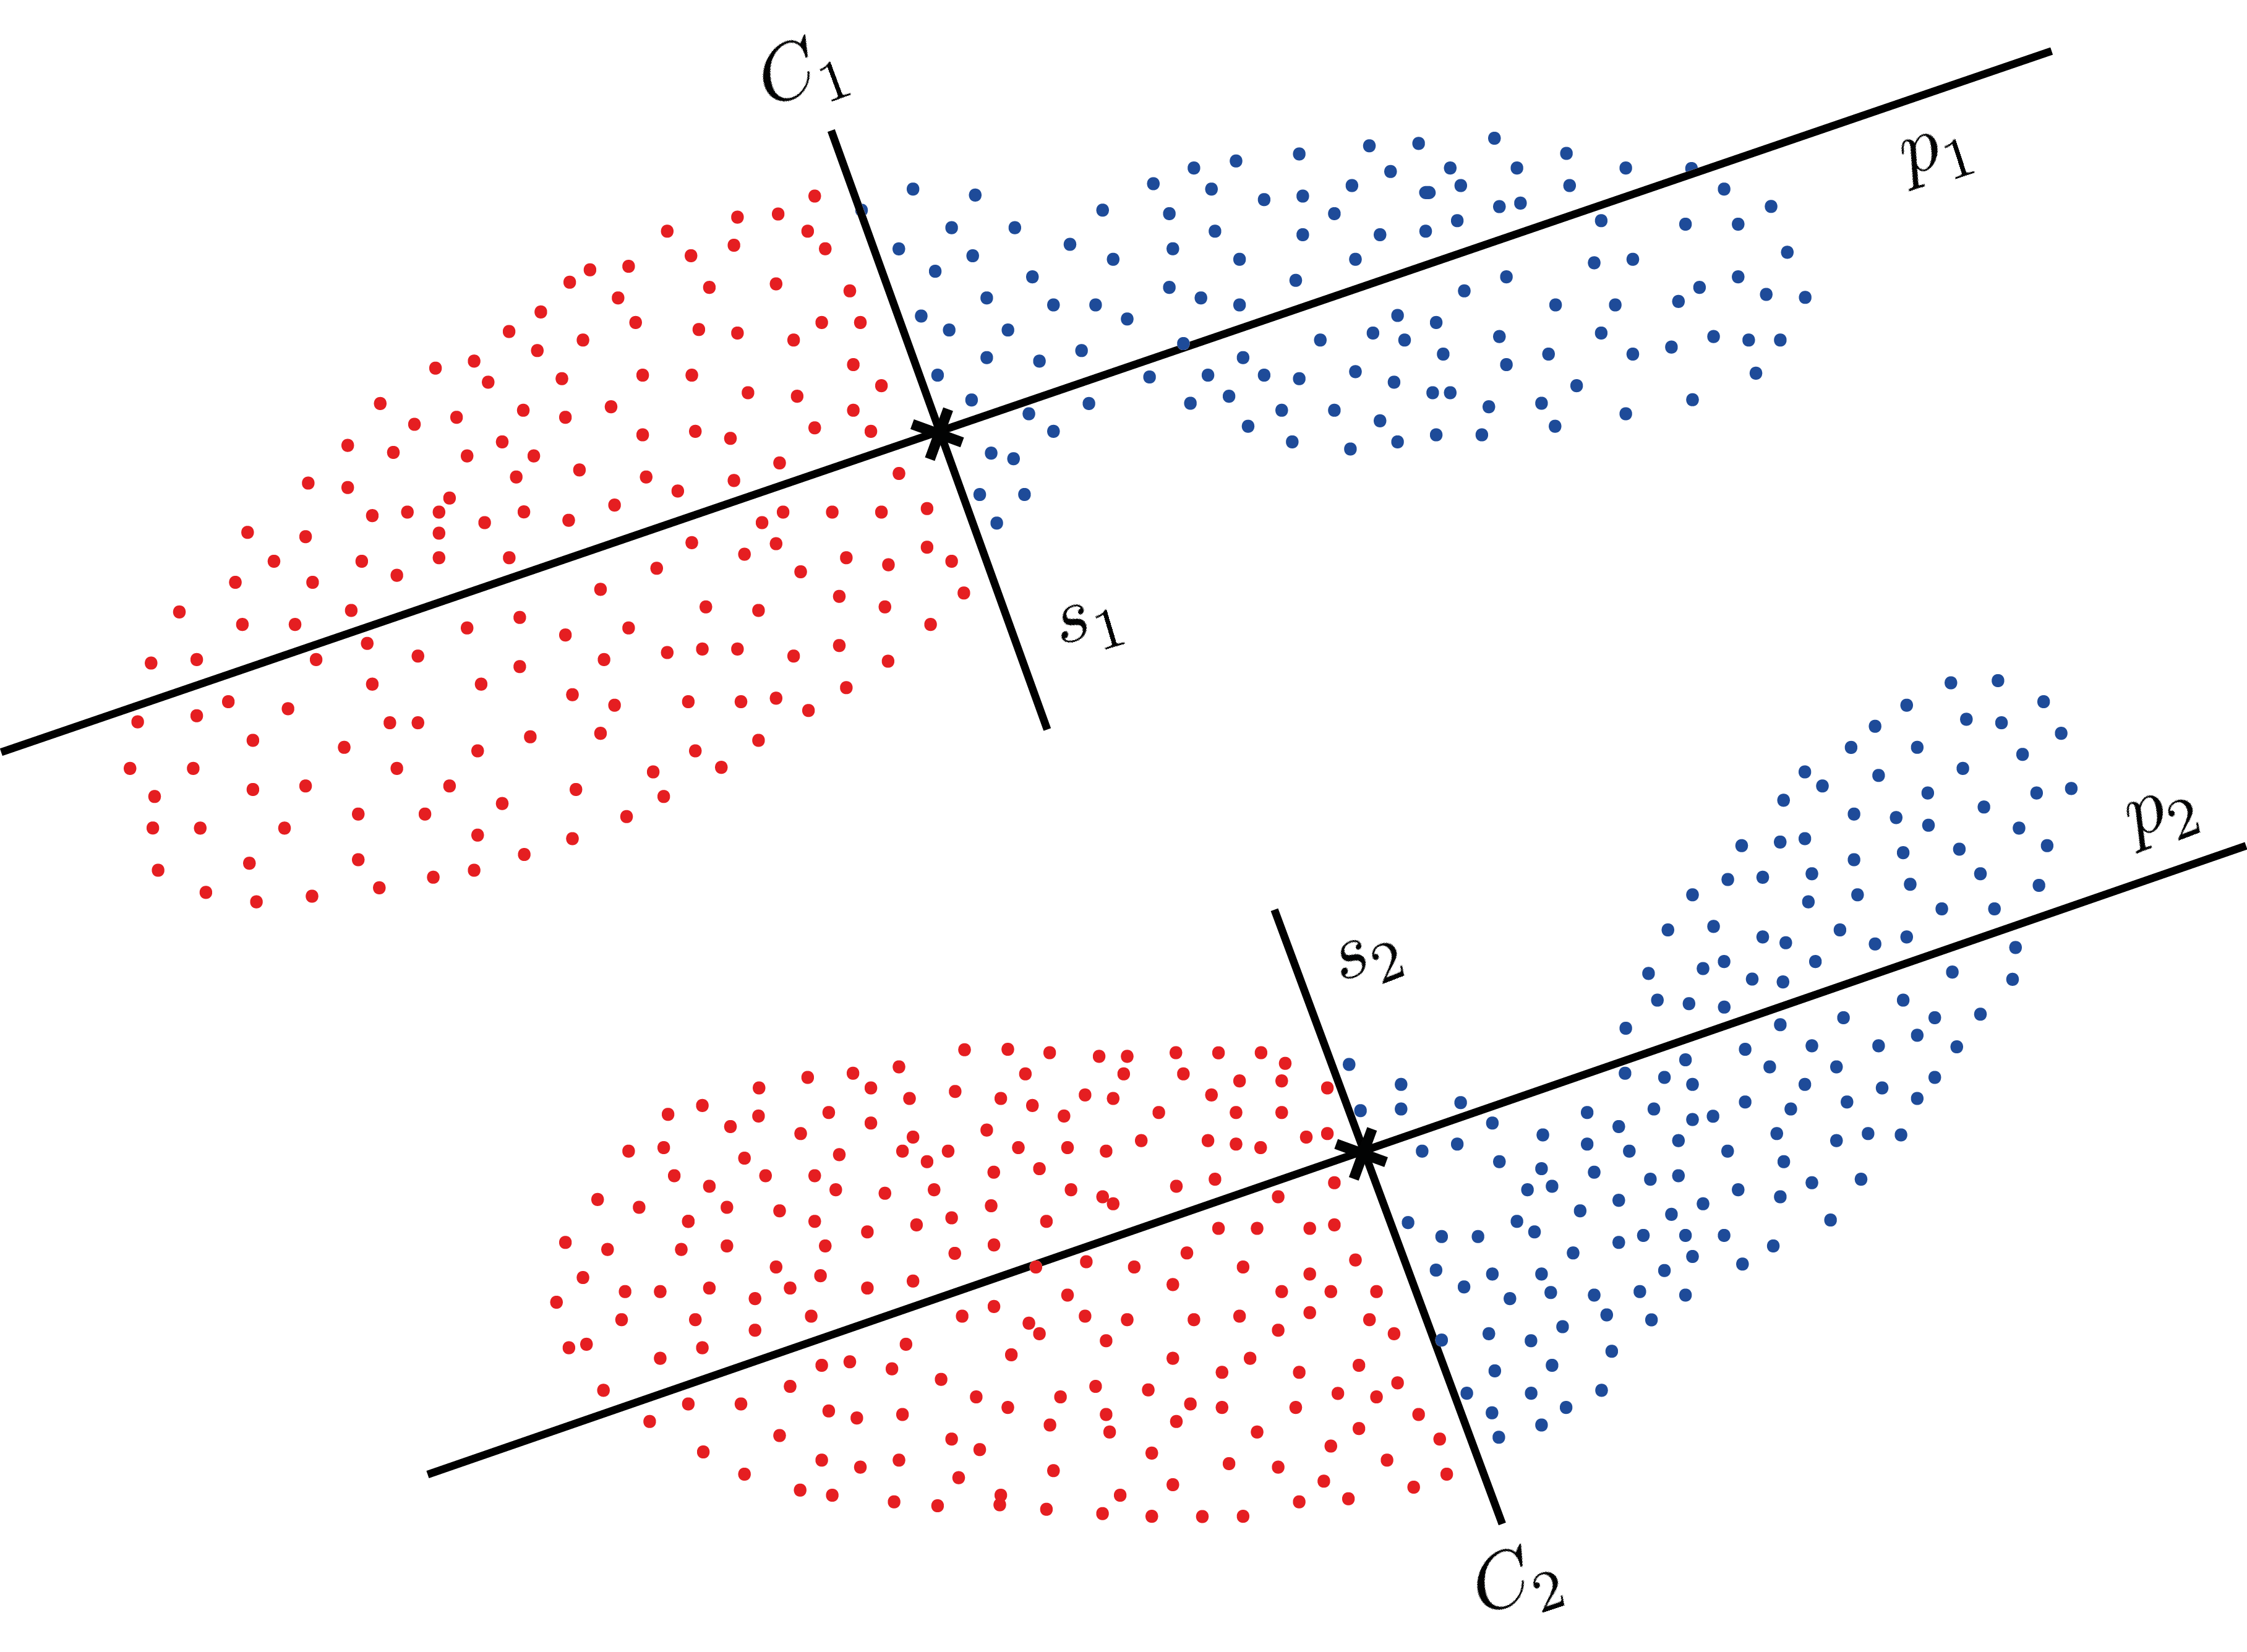
\includegraphics[width=0.8\linewidth]{illustration_axes}
	\caption{Subdividing $C_1$ and $C_2$ into two sub clusters by computing the secondary axes $s_1$ and $s_2$ perpendicular to $p_1$ and $p_2$ through the centroids.}
	\label{fig:dc_axes_2p}
\end{figure}

\subsubsection{Declaring the matching condition between two clusters}

By applying the ICP and the nearest neighbor approach on two associated clusters $C_1$ and $C_2$, a certain matching error $e$ is computed between their cluster points $ C_p =  \{ p_1, \ldots, p_m\}$ and the associated points $ C_q =  \{ q_1, \ldots, q_m\}$. To eliminate the dependency between the matching error and the number of cluster points $m$, the average error per point of $C_p$ and $C_q$
%
\begin{equation}
	e_{\mathrm{avg}(C_p, C_q)} = \frac{1}{| C_p |} \cdot \displaystyle\sum_{i=0}^{m}\| \boldsymbol{p}_i - \boldsymbol{q}_i\|^2
\end{equation}
%
is computed, assuming that the two clusters $C_p$ and $C_q$ contain the same number of cluster points $m$. In case of varying point amounts, the segmentation needs to be carried out differently that sub clusters contain the same number of points. Alternatively, extra points are not considered in the error amount calculation. To declare when two clusters match, it is quite essential to determine an appropriate threshold $\tau$ for the maximum distance $d(p_0, q_0)$ between two associated points $p_0$ and $q_0$. In case of being overvalued, clusters are more likely to match which could result in insufficient subdividing. On the other hand, the clusters are difficult to be matched, which will result in further subdividing and the detection of too many rigid parts. The two clusters $C_p$ and $C_q$ are matching, if $e_{avg} < \tau$.

\subsubsection{Cluster tree}
\label{tree}

The subdividing of the clusters $C_1$ and $C_2$ is realized by a depth-first approach in a tree. Consequently, $C_1$ and $C_2$ represent the root and are subdivided from the left to the right. A node $N$ of the tree contains two related clusters $C_{1,i}$ and $C_{2,i}$, where $i$ defines whether the node is a left ($i=1$) or right ($i=2$) node of the parent. In case of further subdividing, a Node $\mathit{left}$, containing the  clusters $C_{1,i,1}$ and $C_{2,i,1}$, as well as a Node $\mathit{right}$, containing the clusters $C_{1,i,2}$ and $C_{2,i,2}$ origin. If two associated clusters $C_{1,i,j}$ and $C_{2,i,j}$ in a Node $N_i$ match, no further subdividing is performed. The resulting leaves of the tree are the final matching sub clusters and stored from left to right in a list $\mathcal{L} = (L_{1,1},L_{2,1},\ldots,L_{1,m},L_{2,m})$ (see figure \ref{fig:illustrationTree}). By applying the depth-first approach, the neighboring clusters in the list are also neighboring clusters in the main clusters $C_1$ and $C_2$.  As a result, in the following step the adjacent sub clusters of $C_1$ or $C_2$ can be merged (see subsection \ref{mergingClusters}).
\begin{figure}
	\centering
	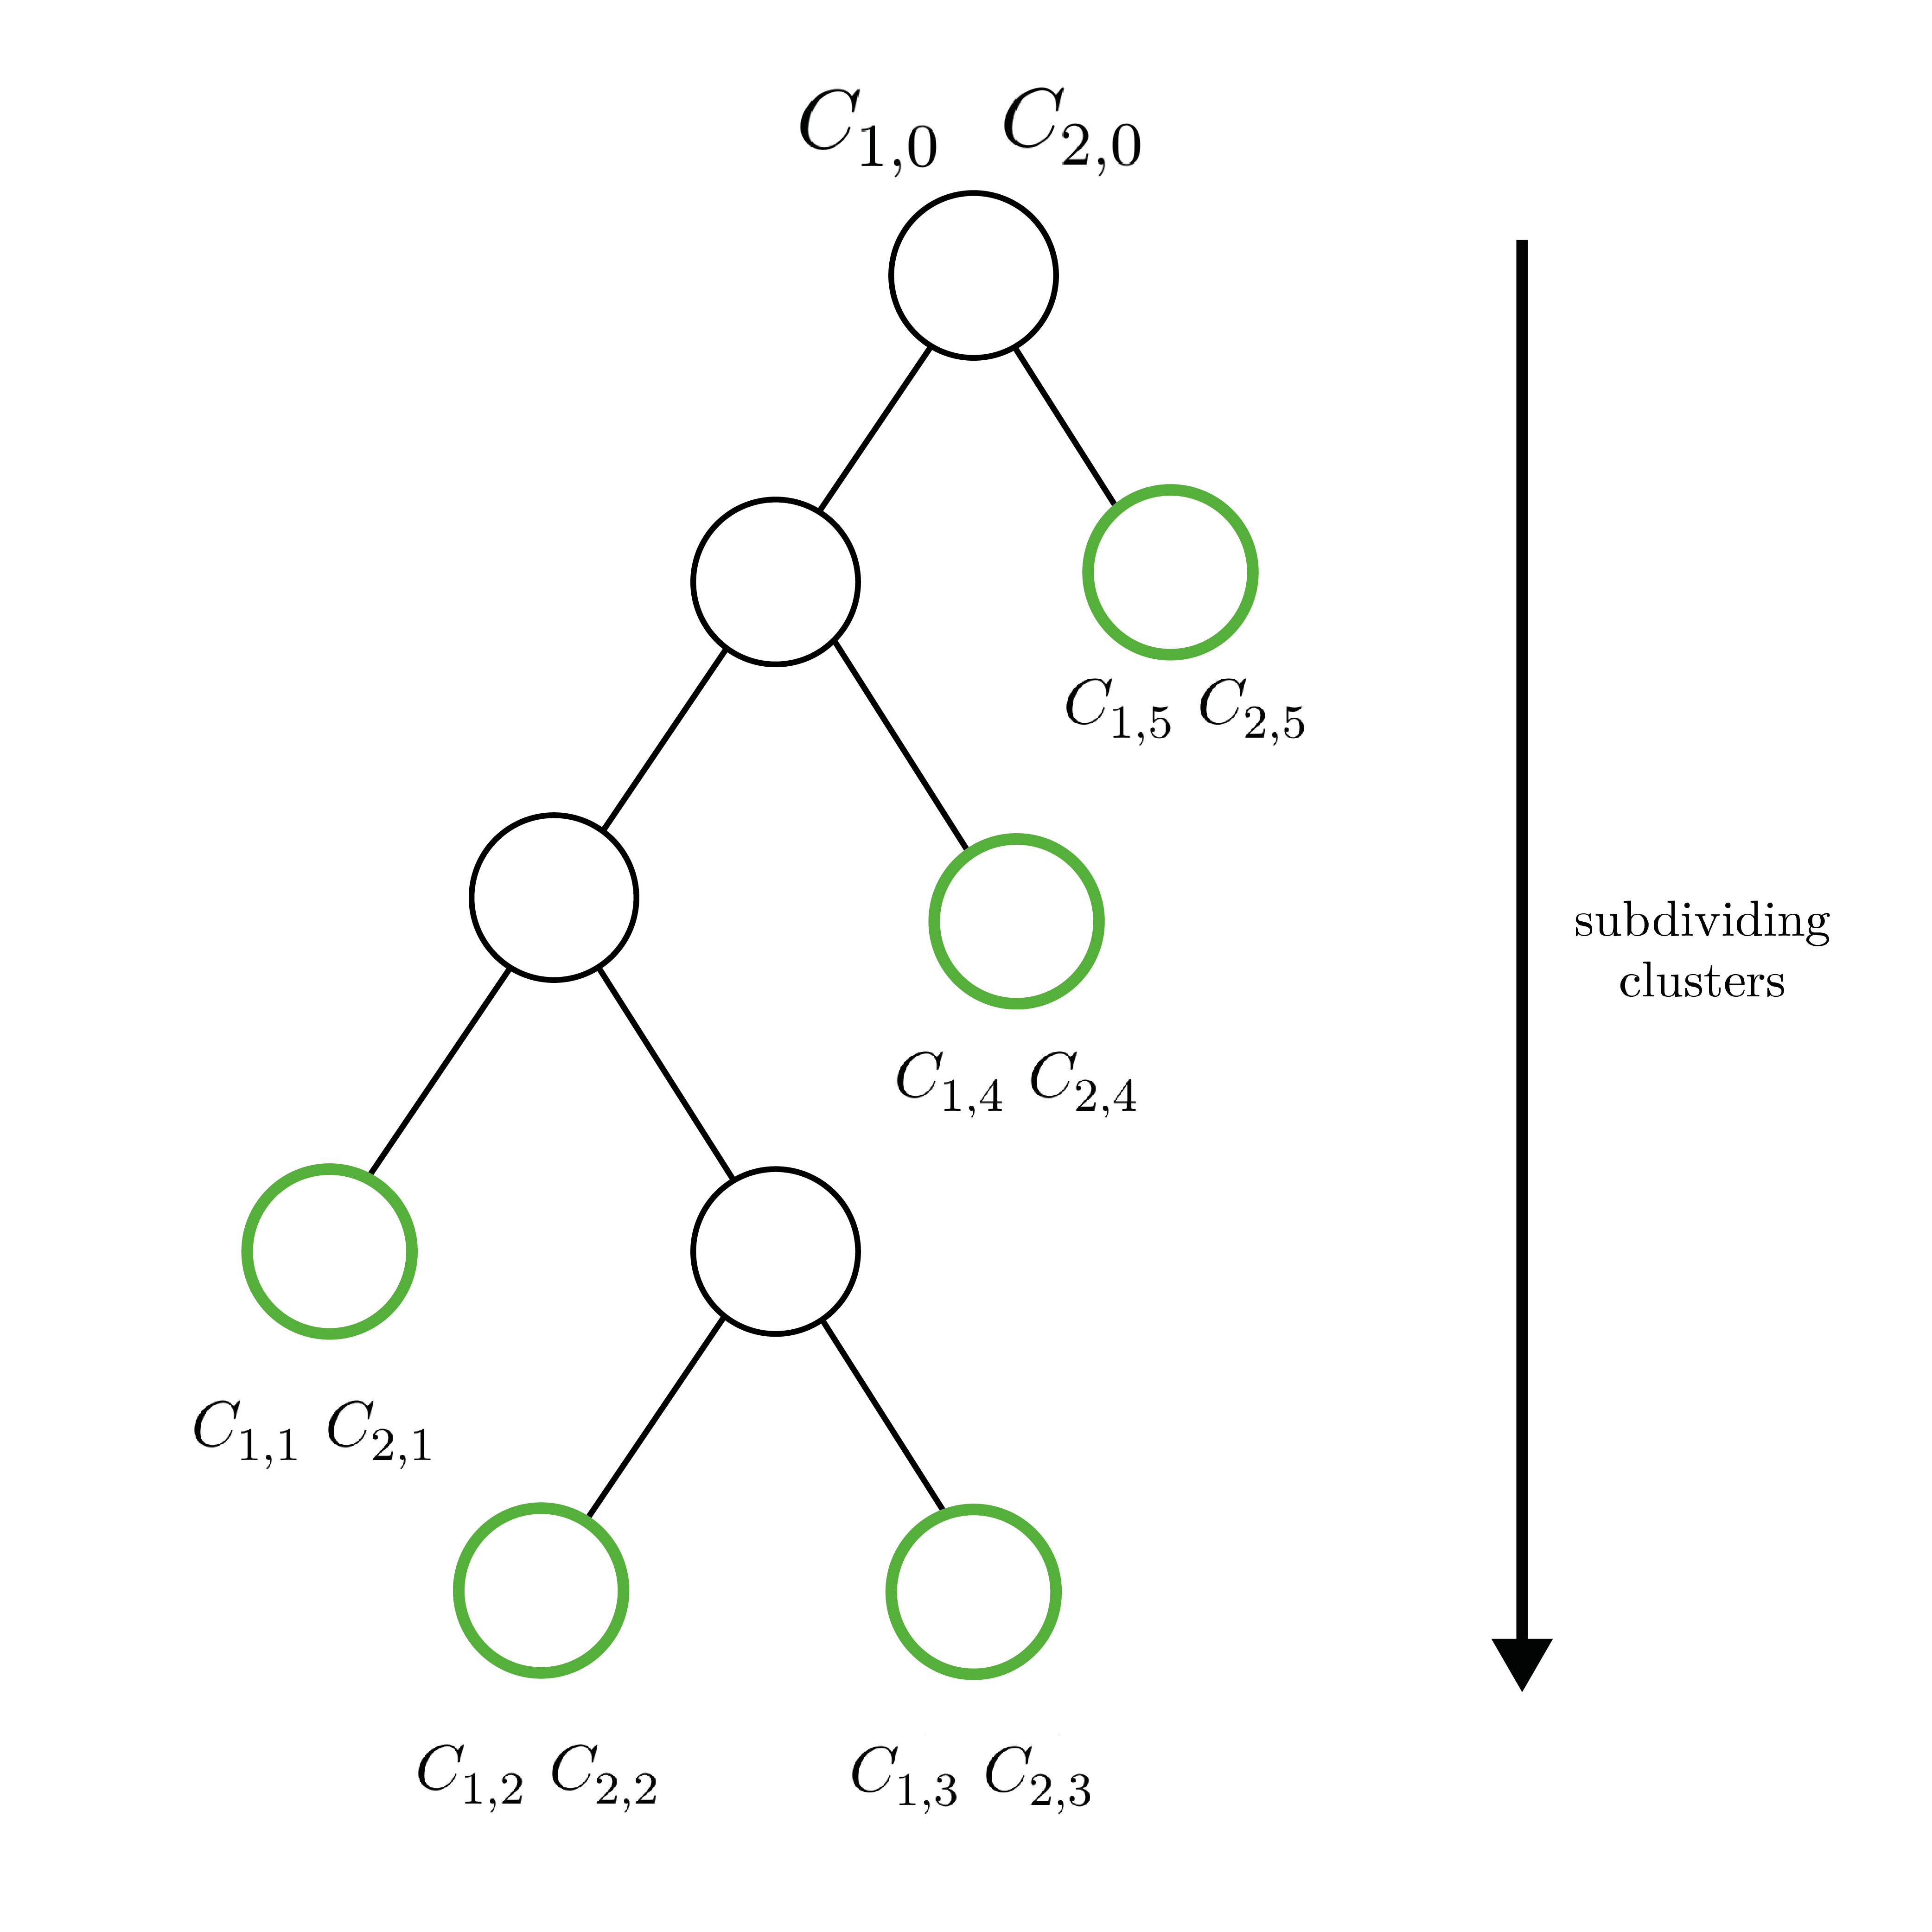
\includegraphics[width=0.7\linewidth]{IllustrationTree}
	\caption{Subdividing of $C_1$ and $C_2$ into matching clusters by a depth-first approach in a tree. The Subdividing terminates if all sub clusters of $C_1$ and $C_2$ match when applying the ICP.}
	\label{fig:illustrationTree}
\end{figure}

\subsection{Merging neighboring clusters to rigid parts}
\label{mergingClusters}x
%%
As a next step, adjacent sub clusters from $\mathcal{L}$ are iteratively merged and subsequently verified to still match. This process is required to rejoin, if necessary, detected sub clusters to the rigid parts of the object. This is the case, if a rigid part was subdivided during the subdividing process (see section \ref{Subdividing}). The merging initiates with the first clusters in the list $L_{1,i}$, $L_{2,i}$ and its adjacent clusters $L_{1,i+1},L_{2,i+1}$. If the resulting merged clusters can be matched, the merging proceeds with the adjacent cluster $L_{1,i+2},C_{2,i+2}$. If not, the merging is not executed and $L_{1,i}$, $L_{2,i}$ are stored in a list of resulting clusters $\mathcal{R}$. The merging procedure then initiates with $L_{1,i+1},L_{2,i+1}$. The process terminates if all clusters of $\mathcal{L}$ are verified and consequently the clusters of $\mathcal{R}$ are assigned to rigid parts $\mathcal{P} =  \{P_1,\ldots,P_m\}$ (see figure \ref{fig:clusterChain}). 

\begin{figure}
	\centering
	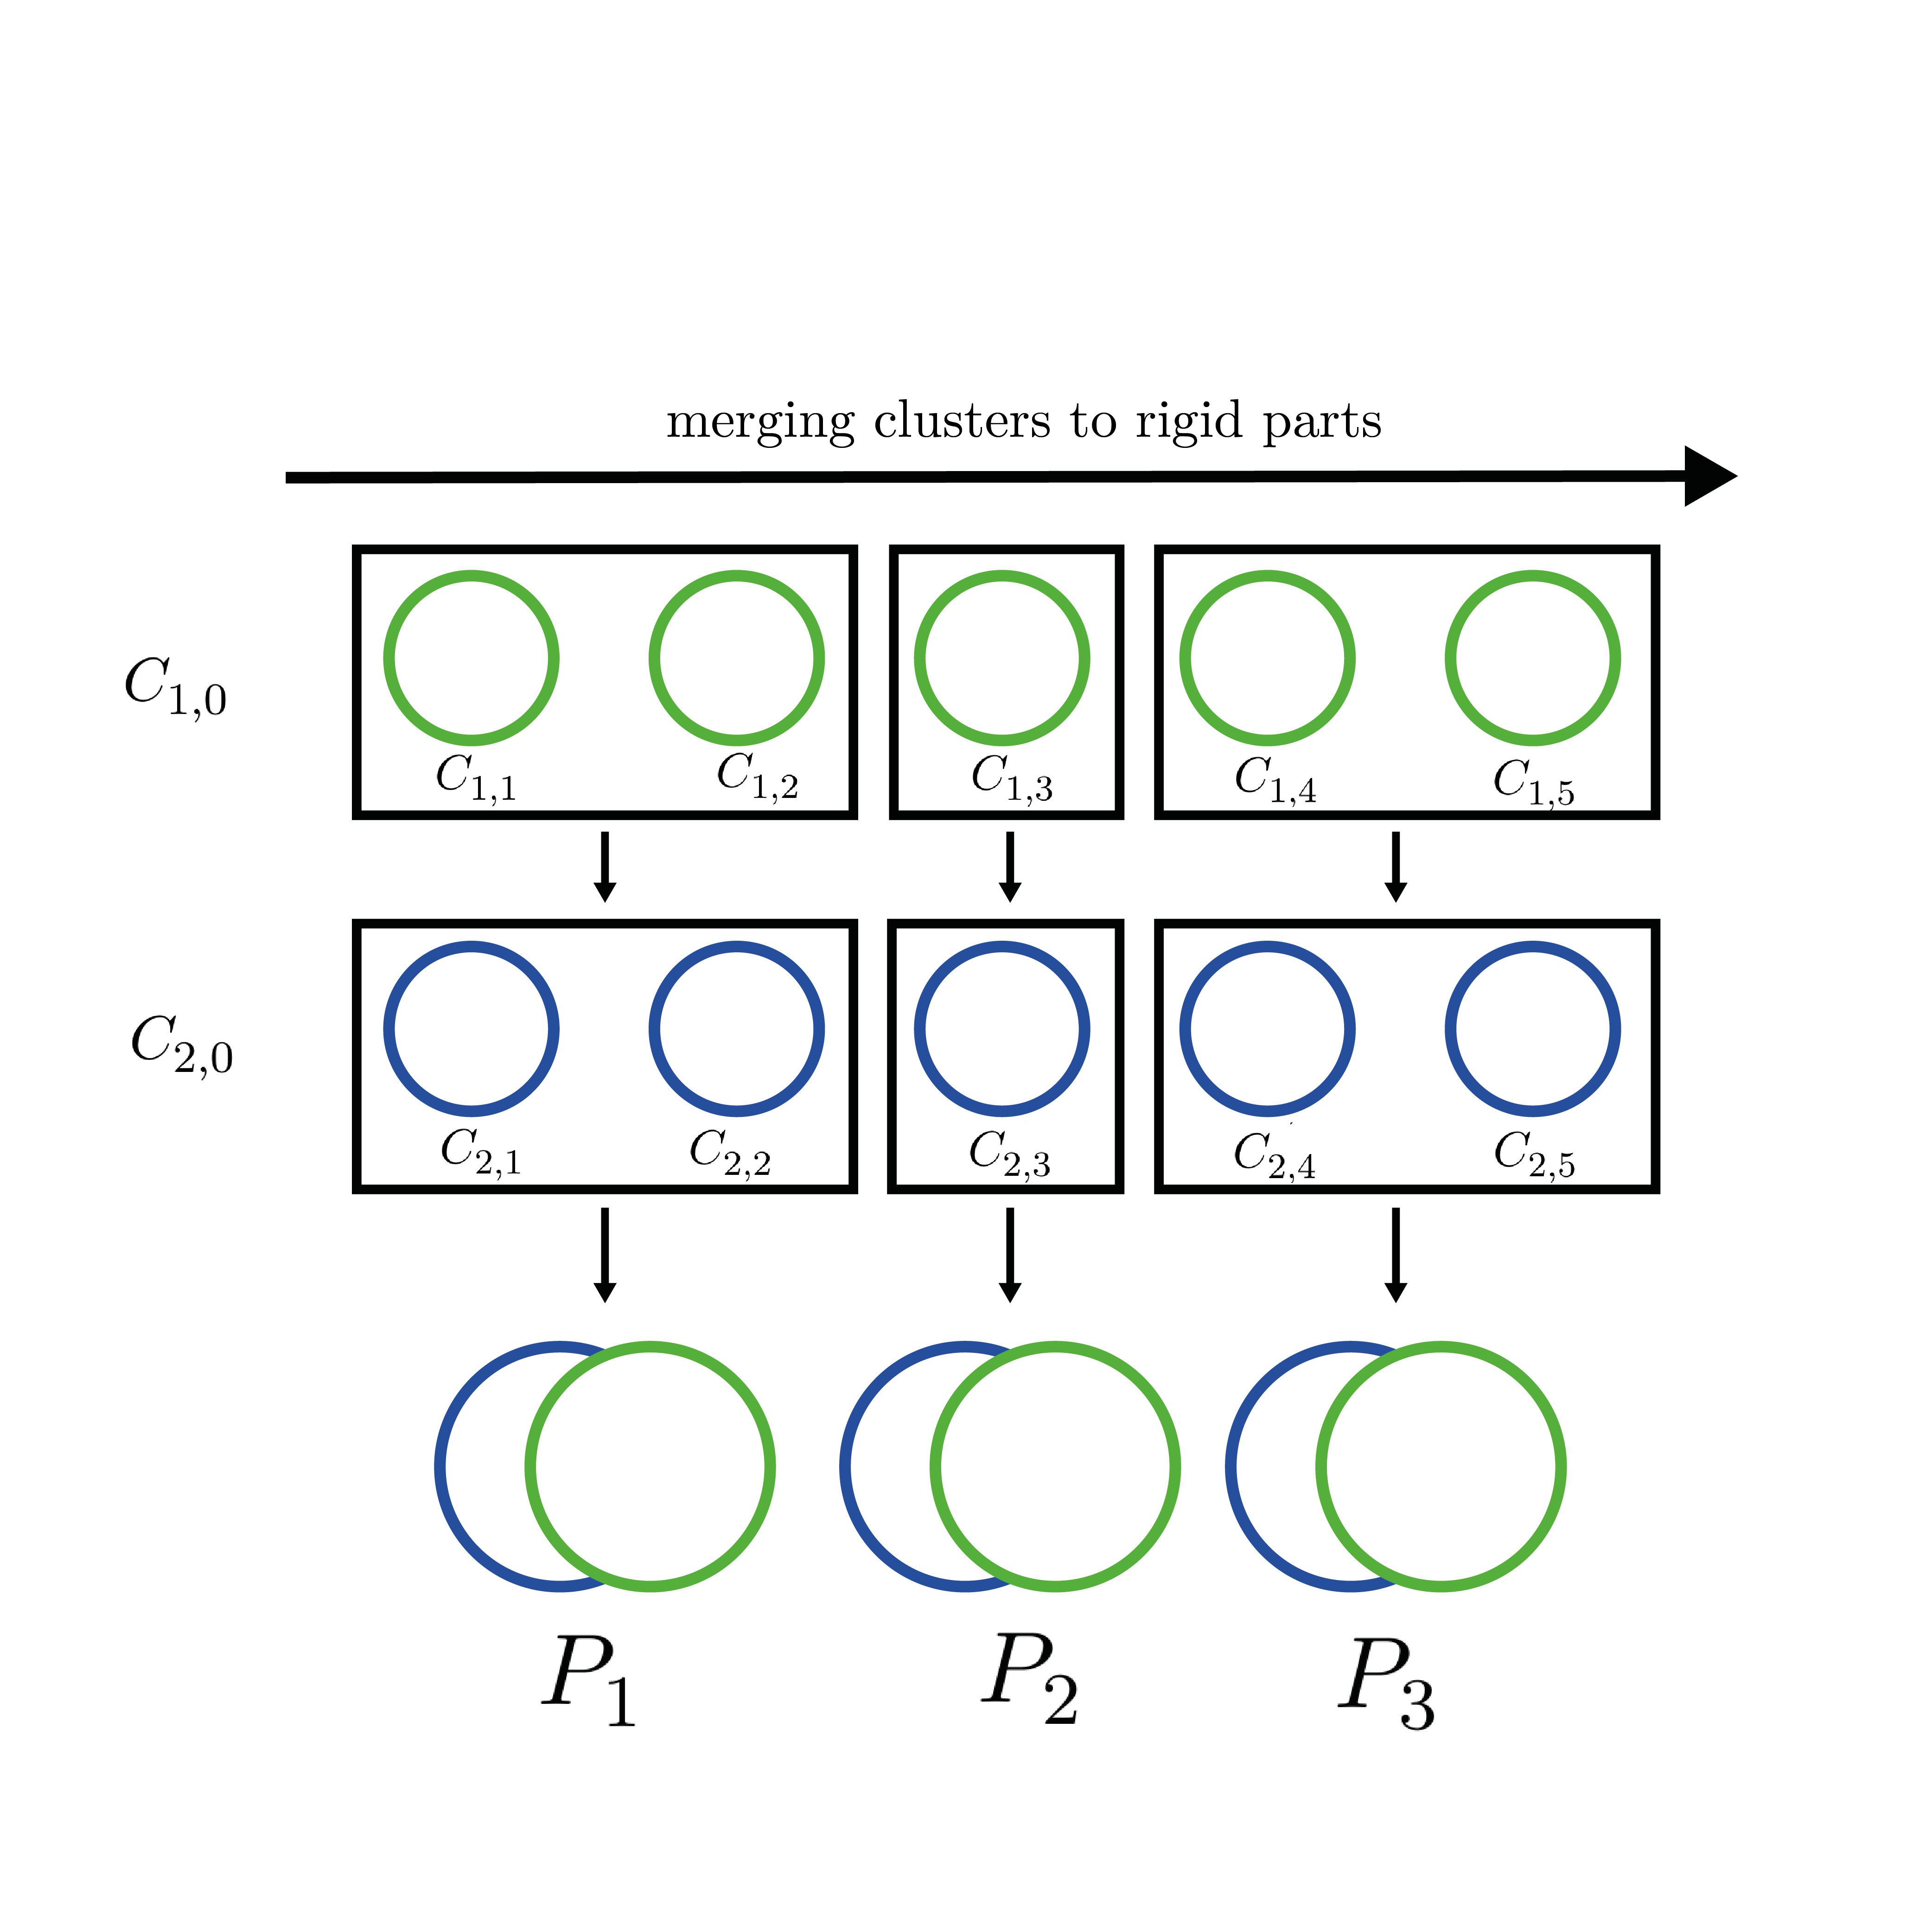
\includegraphics[width=0.8\linewidth]{ClusterChain}
	\caption{Detecting rigid parts of $C_1$ and $C_2$ by iteratively merging adjacent clusters of $\mathcal{L}$ that merged clusters still match.}
	\label{fig:clusterChain}
\end{figure}

\subsection{Joint/skeleton estimation}

After detecting the rigid parts $\mathcal{P} =  \{ {P_1,\ldots,P_m}\}$, they are linked with joints. Their locations are thereby calculated by computing the points of intersection of all principal axis of $\mathcal{P} = \{ {P_1,\ldots,P_m}\}$. However, this calculation assumes that the rigid parts are symmetric, as in the other case the principal axis might not represent the skeleton of an object. For this reason another approach has to be taken into account. Anguelov \cite{Anguelov04} declares joints as two points of two neighboring rigid parts that undergo the same transformation $T$. In the current implementation an object point is only allocated to one rigid part $P$. An improvement of the current situation is therefore to select points that are located near a joint allocated to more neighboring rigid parts and from those selected points the location of a joint is computed. 

\begin{figure}[H]
	\centering\small
	\begin{tabular}{cc}
		\fbox{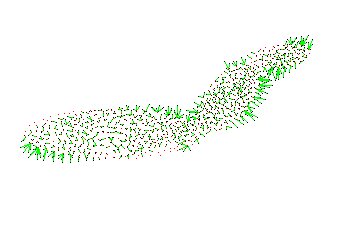
\includegraphics[width=0.45\textwidth]{results/non-rigid_3parts_associations}} &
		\fbox{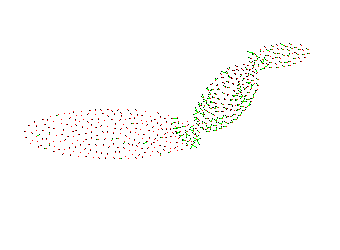
\includegraphics[width=0.45\textwidth]{results/rigid_3parts_associations}} 
		\\
		(a) & (b) 
	\end{tabular}
	\caption{Registration of $C_1$ and $C_2$ before the segmentation into rigid parts (a) and after the segmentation.} 
	\label{fig:ICPResults}
\end{figure}

\section{Implementation}

After planning the algorithm, it was initially implemented and for 2D point clouds, in order to be able to focus solely on developing and testing.

\subsection{Chosen environment}

The initial approach was implemented in Java, using ImageJ as processing library. The chosen environment depends on the following factors:
\begin{itemize}
	\item familiarity and prior experience
	\item complexity
	\item available plug-in for image processing
\end{itemize}
%%
As ImageJ is mainly used for 2D use cases, another implementation would be possible in 3D using PCL in C++. As a result, the attention can be brought to segmentation and visualization in 3D.

\subsection{Architecture}

The initial algorithm was realized with four classes to divide the ``divide and conquer'' algorithm from the Cluster object as well as the Visualization and the registration process of sub clusters.
The main class \texttt{Segmentation} solely requires a stack of two point clouds in 2D. As a first step, possible noise is removed from the input mesh $M$ (see algorithm \ref{alg:noiseRemoval}). The algorithm returns the biggest point cluster $C_i$ that is assumed to be an articulated object. A class \texttt{Cluster} was implemented to store the cluster's points, its centroid, the orientation $\theta$ as well as the principal and secondary axes. For the subdividing, a \texttt{ClusterTree} was implemented to simultaneously divide the main clusters $C_1$ and $C_2$ into sub clusters (see algorithm \ref{alg:subdivide}). Each node $N$ contains thereby two associated clusters $C_{1,i}$ and $C_{2,i}$. For the clustering and merging of clusters a \texttt{List<Clusters>} was used to dynamically add and remove Clusters. Furthermore, a class \texttt{ICP} was created, which takes two clusters to be matched as input, using Procrustes fitting. First, the noise removal and cluster detection is done in the \texttt{Cluster} class. As a next step, the detected main clusters $m$  $C_1,\cdots,C_{m}$ are taken as input with an empty list to get the matching sub clusters of all input clusters. Following, the divide and conquer algorithm (see algorithm \ref{alg:subdivide}) takes advantage of the ICP class to iteratively register two sub clusters of two main clusters $C_{i},\cdots,C_{j}$. As the segmentation is done depth first the verified sub clusters are stored in the list from left to right. The returned segmented list is taken as input to iteratively merge the sub clusters to detected rigid parts (see algorithm \ref{alg:merging}). As a return we get a list with sub clusters representing the rigid parts of the input clusters. Subsequently, the Visualization class is used, to color the cluster points differently and draw PCA related components, like the axis and interference points of different rigid parts.

%TODO: add code snippets for Procrustes...

\begin{figure}
	\centering
	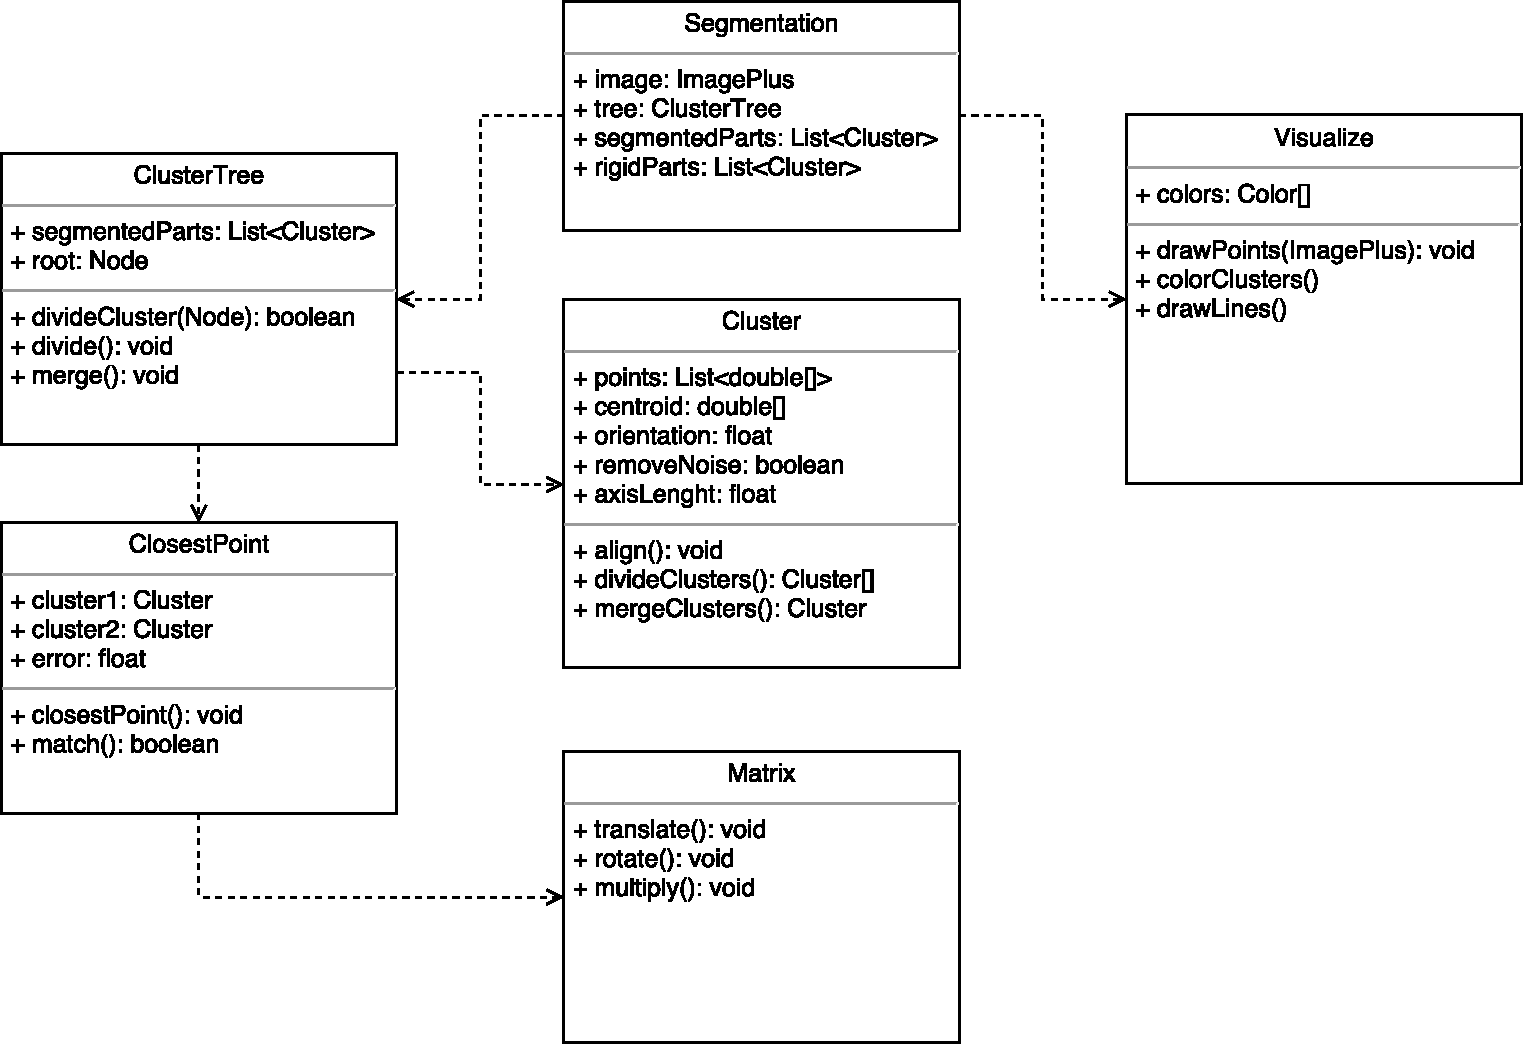
\includegraphics[width=0.9\linewidth]{SegmentationUML}
	\caption{UML diagram of the classes related to the implementation of the algorithm.}
	\label{fig:UML}
\end{figure}

\begin{algorithm}[tbp]
	\caption{Noise removal of an input point mesh $M$ in form a set of unclustered points $\{\boldsymbol{u}_1,\ldots,\boldsymbol{u}_n\}$ by region growing. The first point of $M$ is used as seed and grows a cluster $C_{current}$ by iteratively adding neighboring points located inside a threshold $\tau$. Once, all points have been examined, the largest cluster $C_{max}$ is returned and defined as articulated object to be segmented.}
	
	\begin{algorithmic}[1]     % [1] = all lines are numbered
		\label{noiseRemoval}
		
		\Procedure{RemoveNoise}{$M$} 
		\State $\mathit{C_{max}} \gets ()$
		\State $\mathit{C_{current}} \gets ()$
		\State $n \gets \mathit{sizeOf}(M)$
		\State $m \gets \mathit{sizeOf}(C_{current})$
		
		\While {$n$ > 0}
		\State $\mathit{c_{current}} \gets \mathit{c_{current}} + \boldsymbol{u}_1$
		\For{$i = 1,\ldots,m$}
		\State $M \gets M - C_{current}$
			\For{$j = 1,\ldots,n$}
			\If {\Call{$d$}{$\boldsymbol{p}_i, \boldsymbol{u}_j}< \tau$}
			\State $C_{current} \gets C_{current} + \boldsymbol{u}_j$
			\EndIf
			\EndFor
		\EndFor
		\State $M \gets M - C_{current}$
		\If{$m > \mathit{sizeOf}(C_{max})$}
		\State $C_{max} \gets C_{current}$
		\EndIf
		\State $C_{current} \gets ()$
		\EndWhile
		\State\Return $C_{max}$
		\EndProcedure	
	\end{algorithmic}
\end{algorithm}

\begin{algorithm}[tbp]
	\caption{Recursive subdividing of two clusters $C_1$ and $C_2$, in the form of a Node $\mathit{N}$ in a Tree, into matching sub clusters. The ICP is applied on two corresponding clusters in $\mathit{N}$ to verify them to match, in which case they are stored in a list. Otherwise, if the two clusters do not match, they are further subdivided. The list with all matching subclusters is returned once the subdivide algorithm terminates.}
	\label{alg:subdivide}
	
		\begin{algorithmic}[1]     % [1] = all lines are numbered
			\label{clusterTree}
			\Procedure{ClusterTree}{$\mathit{C_1}, \mathit{C_2}$}
			
			\State $L \gets ()$
			\State $\mathit{left} \gets \mathit{nil}$
			\State $\mathit{right} \gets \mathit{nil}$
			\State $N \gets \langle C_1, C_2, \mathit{left}, \mathit{right}\rangle$
			\State $L \gets \Call{Subdivide}{N}$
			\State $P \gets \Call{MergeClusters}{L}$
			
			\EndProcedure
		\end{algorithmic}
	
	\begin{algorithmic}[1]     % [1] = all lines are numbered
		\label{subdivide}
		\Procedure{Subdivide}{$N$}
		
		\If {$\Call{match}{C_1(N)}, C_2(N)$}
		\Comment{Apply ICP on two clusters}
		\State $L \gets L + (N)$
		
		\Else
		\State $\mathit{left}(N) \gets \Call{Split}{N}$
		\State $\mathit{right}(N) \gets \Call{Split}{N}$
		\Comment{Split the cluster into a left and right side}
		\State \Call{Subdivide}{$\mathit{left}(N)$}
		\State \Call{Subdivide}{$\mathit{right}(N)$}
		\Comment{Recall the algorithm with sub clusters}
		\EndIf
		
		\State\Return $L$
		\Comment{Return all sub clusters after termination.}
		\EndProcedure
			
	\end{algorithmic}
\end{algorithm}

\begin{algorithm}[tbp]
	\caption{Merging of the sub clusters $\mathit{L} = ((L_{1,1}, L_{2,1}),\ldots,(L_{1,m}, L_{2,m}))$, resulting from algorithm \ref{alg:subdivide} in the order of being stored, to rigid parts $\mathcal{P}$. Verify the matching of merged adjacent clusters $L_{i,j}$ and $L_{i,j+1}$ from $C_1$ and $C_2$. The merging is continued until no match can be done. In this case the last last merged cluster pairs are stored as rigid parts $P_1$ and $P_2$. The algorithm then continues with the next cluster pair in the list and terminates if all pairs have been traversed. The list with all detected rigid parts $\mathcal{P}$ is returned.}
	\label{alg:merging}
	
	\begin{algorithmic}[1]     % [1] = all lines are numbered
		\label{merging}

		\Procedure{MergeClusters}{$L$} 
		\State $P \gets ()$
		\State $P_1 \gets L_{1,1}$
		\State $P_2 \gets L_{2,1}$
		\State $n \gets \mathit{sizeOf}(L)$
		
		\For{$i = 2,\ldots,n$}
		\State $\mathit{merge_1} \gets \Call{Merge}{P_1, L_{1,i}}$
		\State $\mathit{merge_2} \gets \Call{Merge}{P_2, L_{2,i}}$
		
		\If {\Call{match}{$merge_1$, $merge_2$}}
		\Comment{Apply ICP on two merged clusters}
		\State $\mathit{P_1} \gets merge_1$
		\State $\mathit{P_2} \gets merge_2$
		\Comment{Continue merging with merged clusters}
		\Else
		\State $P \gets P + (P_1, P_2)$
		\State $P_1 \gets L_{1,i}$
		\State $P_2 \gets L_{2,i}$
		\Comment{Initiate merging with current clusters}
		\EndIf
		\EndFor
		\State $P \gets P + (merge_1, merge_2)$
		\State\Return $P$
		\EndProcedure	
	\end{algorithmic}
\end{algorithm}

\section{Results}

At first, the implementation was tested on two point clouds of an articulated object with only two rigid parts. The segmentation results are directly dependent on the matching error threshold $\tau$ which can bee seen on table \ref{table:segmentation_results}. The higher the threshold $\tau$, the less clusters and subsequently rigid parts can be detected, as two clusters are more likely to match and are not further subdivided. The lower $\tau$, the more clusters and rigid parts will be detected, as clusters require further subdividing in order to match. Figure \ref{fig:2rigidParts} and figure \ref{fig:3rigidParts} show the clustering and rigid part detection of two simple objects, in regard to their rigid parts linked like a chain. For those objects, with a threshold $\tau = 5$ the right number of rigid parts is detected. However, the segmentation position does not correspond to the actual joint of $C_1$ and $C_2$. The reason is, that the average error $e_{avg}$ is computed without any weighting of points. Especially points located near a joint need to be treated cautiously. Figure \ref{fig:4rigidParts} shows a more complex object.
%%
\begin{table}
	\centering\small
	\begin{tabular}{ |c|c|c|c| } 
		\hline
		Rigid parts & $\tau$ & detected clusters & detected rigid parts \\
		\hline
		& 3 & 21 & 14 \\ 
		2& 5 & 3 & 2 \\
		& 7 & 2 & 2 \\
		\hline
		& 4 & 38 & 31 \\ 
		3 & 6 & 4 & 3 \\
		& 8 & 3 & 3 \\
		\hline
		& 6 & 35 & 26 \\ 
		4 & 7 & 3 & 3 \\
		& 8 & 3 & 3 \\
		\hline
	\end{tabular}
	\caption{Segmentation results}
	\label{table:segmentation_results}
\end{table}
%%
\begin{figure}
	\centering\small
	\begin{tabular}{@{}c@{\hspace{2mm}}c@{}} % mittlerer Abstand = 12mm
		\fbox{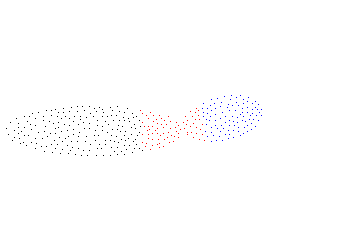
\includegraphics[width=.40\textwidth]{results/2_1parts_clusters_2th}} &
		\fbox{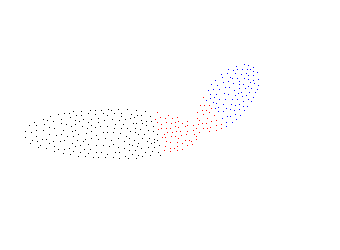
\includegraphics[width=.40\textwidth]{results/2_2parts_clusters_2th}} 
		\\
		(a) & (b)
		\\[4pt]	%vertical extra spacing (4 points)
		\fbox{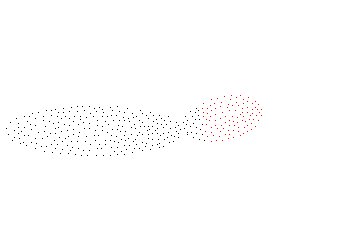
\includegraphics[width=.40\textwidth]{results/2_1parts_rigidParts_2th}} &
		\fbox{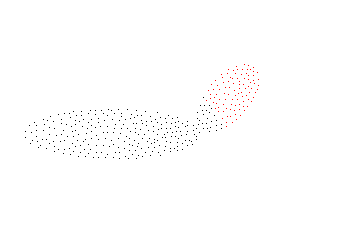
\includegraphics[width=.40\textwidth]{results/2_2parts_rigidParts_2th}} 
		\\
		(c) & (d)
	\end{tabular}
	\caption{Taking a Mesh $M$ in two poses with only two rigid parts as input, with a threshold $\tau = 5$, 3 clusters are detected in $C_1$~(a) and $C_2$~(b),
		which results in 2 rigid parts in $C_1$~(c) and $C_2$~(d).}
	\label{fig:2rigidParts}
\end{figure}
%%
\begin{figure}
	\centering\small
	\begin{tabular}{@{}c@{\hspace{2mm}}c@{}} % mittlerer Abstand = 12mm
		\fbox{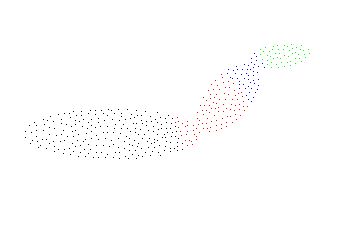
\includegraphics[width=.40\textwidth]{results/3_1parts_clusters_2th}} &
		\fbox{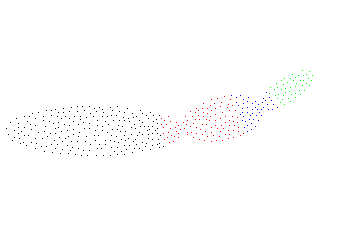
\includegraphics[width=.40\textwidth]{results/3_2parts_clusters_2th}} 
		\\
		(a) & (b)
		\\[4pt]	%vertical extra spacing (4 points)
		\fbox{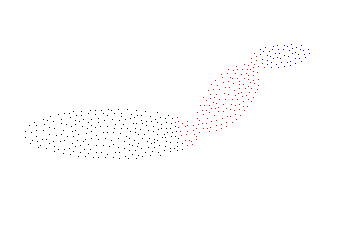
\includegraphics[width=.40\textwidth]{results/3_1parts_rigidParts_2th}} &
		\fbox{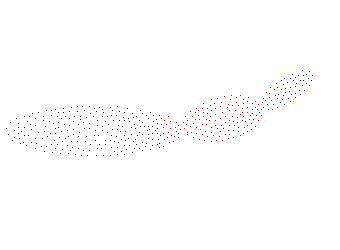
\includegraphics[width=.40\textwidth]{results/3_2parts_rigidParts_2th}} 
		\\
		(c) & (d)
	\end{tabular}
	\caption{Taking a Mesh $M$ in two poses with three rigid parts as an input, with a threshold $\tau = 6$, 4 clusters are detected in $C_1$~(a) and $C_2$~(b),
		which results in 3 rigid parts in $C_1$~(c) and $C_2$~(d).}
	\label{fig:3rigidParts}
\end{figure}
The segmentation into rigid parts is also apparent, when visualizing the point registration between $C_1$ and $C_2$ (see figure \ref{fig:ICPResults}). Two associated points from $C_1$ and $C_2$ are thereby linked with green lines. Comparing the registration results before and after a segmentation into rigid parts clearly shows, that the registration of rigid parts with the ICP results in a lower matching error $e$.
%%	
\begin{figure}[H]
	\centering\small
	\begin{tabular}{cc}
		\fbox{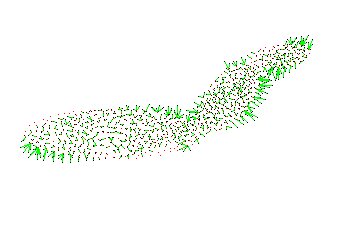
\includegraphics[width=0.45\textwidth]{results/non-rigid_3parts_associations}} &	
		\fbox{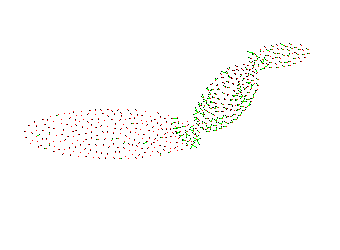
\includegraphics[width=0.45\textwidth]{results/rigid_3parts_associations}} 
		\\
		(a) & (b) 
	\end{tabular}
	\caption{Registration of $C_1$ and $C_2$ before the segmentation into rigid parts (a) and after the segmentation (b).} 
	\label{fig:ICPResults}
\end{figure}
%%		
In case of a more complex object, the simple segmentation algorithm fails. Although varying threshold $\tau$ for the matching, there are either too many or few rigid parts detected. When using $\tau = 7$ (see figure \ref{fig:4rigidPartsHighTH}) only 3 clusters and rigid parts can be detected. By decreasing $\tau$ to 6 (see Figure \ref{fig:4rigidParts}), further subdividing is done, which leads to a too high number of rigid parts and clusters.
%%
\begin{figure}[H]
	\centering\small
	\begin{tabular}{cc}
		\fbox{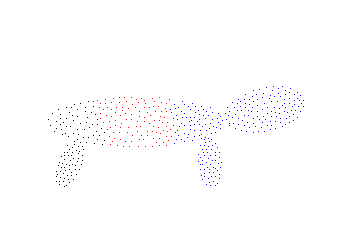
\includegraphics[width=0.45\textwidth]{results/4_1parts_clusters_rigidParts_7th}} &	
		\fbox{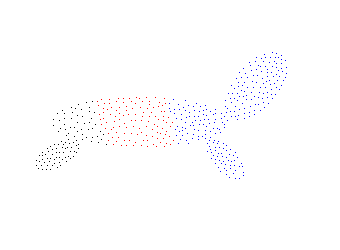
\includegraphics[width=0.45\textwidth]{results/4_2parts_clusters_rigidParts_7th}} 
		\\
		(a) & (b) 
	\end{tabular}
	\caption{Taking a more complex Mesh $M$ in two poses with four rigid parts as an input, with a threshold $\tau = 7$, 3 clusters and rigid parts can be detected in $C_1$~(a) and $C_2$~(b).} 
	\label{fig:4rigidPartsHighTH}
\end{figure}
\begin{figure}[H]
	\centering\small
	\begin{tabular}{@{}c@{\hspace{2mm}}c@{}} % mittlerer Abstand = 12mm
		\fbox{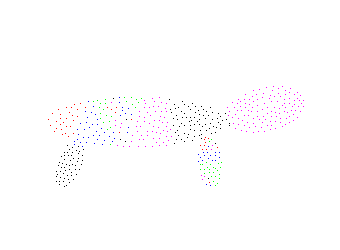
\includegraphics[width=.40\textwidth]{results/4_2parts_clusters_6th}} &
		\fbox{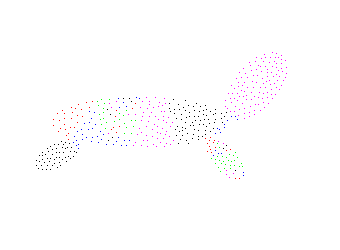
\includegraphics[width=.40\textwidth]{results/4_1parts_clusters_6th}} 
		\\
		(a) & (b)
		\\[4pt]	%vertical extra spacing (4 points)
		\fbox{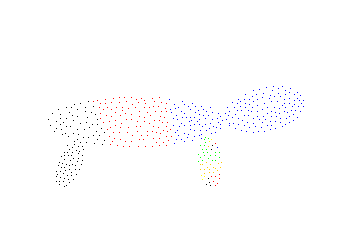
\includegraphics[width=.40\textwidth]{results/4_1parts_rigidParts_6th}} &
		\fbox{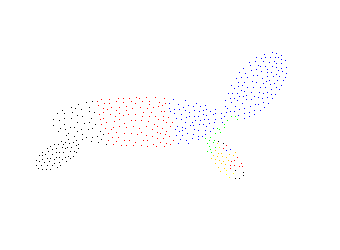
\includegraphics[width=.40\textwidth]{results/4_2parts_rigidParts_6th}} 
		\\
		(c) & (d)
	\end{tabular}
	\caption{Taking a more complex Mesh $M$ in two poses with four rigid parts as an input, with a threshold $\tau = 6$ , 35 clusters are detected in $C_1$~(a) and $C_2$~(b),
		which results in 26 rigid parts in $C_1$~(c) and $C_2$~(d).}
	\label{fig:4rigidParts}
\end{figure}	
The algorithm generally works for simple objects, in which the rigid parts are linked like a chain. Still, the segmentation location is not accurate, which might be disposed by introducing weights to points located near a joint. For more complex object with a skeleton structure, e.g. a human, where one rigid part is linked to more than two rigid parts, this simple implementation fails. In this case, another approach has to be found, as a skeleton structure is more complex to extract than a simple chain structure.

\section{Improvements}

In case of articulated objects with a skeleton structure, the segmentation algorithm in its simple form fails. The main reasons are the following:
%%
\begin{itemize}
	\item By recursively subdividing $C_1$ and $C_2$ the detected sub clusters might actually count to more than one and being located apart from each other. 
	\item In case of a matching cluster being a part of a rigid part, no further operations are done with the match. The rigid part is anticipated to be generated by merging neighboring sub clusters.
	\item By further sub dividing clusters, the merging becomes more difficult, as the clusters are scattered next to each other.
	\item The detection of joints is not exact although the segmentation in the approximate rigid parts succeeds as sub clusters are good enough to fit, but still there might be better fits with less or more points.
\end{itemize}
%%
Thus, the initial approach needs to be extended, which solved the issues being mentioned.

\subsection{Region growing}
During the segmentation of an object in two different poses, there is the general case that the divided parts being compared do not contain the same number of points. As this state might come to undesirable matching errors, parts with the same sizes could be generated by region growing. This can be e.g. implemented by starting with the most outside point of two poses and grow regions with the same size of points which are then compared. Furthermore, the detection of multiple clusters can be treated, in case of subdividing clusters. The detected clusters are as a result treated individually.

\subsection{Matching error}
Another improvement is the assurance that during the ICP procedure each point only has one nearest neighbor and also considering the case, that there are not always the same amount of points in two clusters (uneven number of points). By doing so, not all points would contribute to the matching error. Furthermore, weights should be added to the points, especially points located near a joint should be treated cautiously. A cluster could be therefore further subdivided, if a minimum number of points is above the error threshold $\tau$ and not the average. 

\subsection{Initial alignment of clusters}
The initial ``Divide and Conquer'' approach is used to detect two matching sub clusters of $C_1$ and $C_2$. But unlike previous implementations, the rigid parts are not detected by a following merging step, but by region growing, until the matching error $e$ is above the specified threshold $\tau$.
If a rigid part is detected, it is stored and the same procedures initiates with the other points of $C_1$ and $C_2$. By doing so, all rigid parts are sequentially detected from one direction to the other.

%\subsection{Error handling}
%The region growing procedure needs to terminate if points of another rigid part are added. Following, a higher matching error $e$ is detected. To guarantee successful rigid part detection this procedure premises that the regions in two comparing sub clusters grow the same way, otherwise the region growing might terminate before detecting the whole rigid part. 

\subsection{Segmentation of articulated objects}
The most crucial deficit  of the proposed algorithm is that is does not work with articulated objects, whose parts are not simple linked as a chain, but a rigid part can have more than two linking rigid parts. An example would be the skeleton of humans and most animals. As a result, the objects are simply too complex to linearly subdivide them. One improvement proposition is thereby the initial alignment of the object, that the largest rigid part is aligned.  A similar approach was taken during the LRP algorithm \cite{guo2016correspondence}. Then, recursively linked parts of this largest rigid part are detected (see section \ref{LRP}).

\subsection{ICP}
Sparse correspondences of two input clusters $C_i$ and $C_j$ were initially achieved by applying the Iterative closest point algorithm. Thereby, the two input clusters are aligned by means of the PCA. Following, corresponding points of $C_i$ and $C_j$ are only considered, if they are \textit{reciprocal} (see subsection \ref{functionalityLRP}). Furthermore, the euclidean distance between two cluster points $d(\boldsymbol{p}_i,\boldsymbol{p}_j)$ must be below a predefined threshold $\tau$. As a consequence, points being located far away from each other do not contribute to the alignment of $C_i$ and $C_j$ and are not stored as correspondence. Those are assumed to be small rigid parts with different transformations.
